\subsection{Methodology}

We propose a methodology to demystify GPU microarchitecture features and correlate them with performance. 
The workflow consists of three major components: CUDA binary tools, a instruction solver, and meticulously benchmarking\jled{(because it is a benchmarking process not just build and use a benchmark)}, and two program sets: sample programs and microbenchmark.
% a deliberate microbenchmark
Each sample program is a synthetic PTX file which generates specific instructions as our reference in the instruction solver. \jled{xiuxia, check correctness}
Deliberate microbenchmark is designed for the assembler to tune code at assembly language level, to find the correlation between microarchitecture and performance.
We dissemble a binary library (such as cuBLAS) to provide a high coverage of instructions to instruction solver.
We use cuBLAS in this work since it contains nearly all needed instructions for SGEMM routine. 

We first leverage CUDA binary tools ({\tt cuobjdump} and {\tt nvdiasm}) to disassemble ASM codes from sample programs and the library. 
% A library might provide a high coverage of instruction sets. 
As introduced in section~\ref{sec:cuda}, these generated assembly files ({\em sass}) provide a instruction encoded number to be cracked.
Our instruction solver takes the assembly files as input to decode each $64$-bit binary instruction. 
We design a set of algorithms to solve all fields of a binary instruction. 
These fields include various {\em operands}, {\em opcodes} and {\em modifiers}. The solver retrieves the undocumented ISA specification, which is used to implement an native assembler. Then, we design deliberate microbenchmarks and leverage the assembler to tune code at assembly language level. In the end, the tuning process will lead to some practical observations on the correlation between microarchitecture and performance.

\begin{figure}[htbp]
\begin{center}
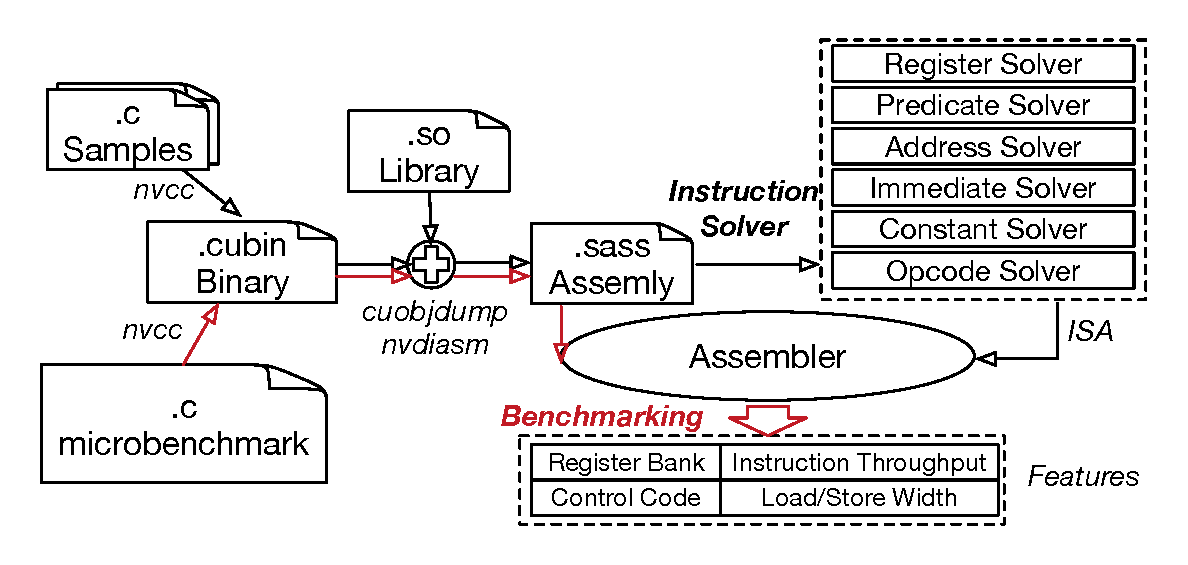
\includegraphics[scale=0.45]{methodology}
\caption{A schematic diagram of demystifying GPU microarchitecture features by leveraging CUDA binary tools. The black arrows represent the workflow of instruction solver while the red ones represents benchmarking to find out correlation between microarchitecture and performance.\jled{`Assembly' to `ASM', `Samples' to `Nanobenchmark'}}
\label{fig:workflow}
\end{center}
\end{figure}


